% REV01 Wed 23 Jun 2021 06:48:06 WIB
% START Tue 04 May 2021 13:55:16 WIB

\chapter{A SOLO AND A DUETT}

The wind was blowing so hard when the visitor came out at the shop-door
into the darkness and dirt of Limehouse Hole, that it almost blew him
in again. Doors were slamming violently, lamps were flickering or blown
out, signs were rocking in their frames, the water of the kennels,
wind-dispersed, flew about in drops like rain. Indifferent to the
weather, and even preferring it to better weather for its clearance of
the streets, the man looked about him with a scrutinizing glance. ‘Thus
much I know,’ he murmured. ‘I have never been here since that night, and
never was here before that night, but thus much I recognize. I wonder
which way did we take when we came out of that shop. We turned to the
right as I have turned, but I can recall no more. Did we go by this
alley? Or down that little lane?’

He tried both, but both confused him equally, and he came straying
back to the same spot. ‘I remember there were poles pushed out of upper
windows on which clothes were drying, and I remember a low public-house,
and the sound flowing down a narrow passage belonging to it of the
scraping of a fiddle and the shuffling of feet. But here are all these
things in the lane, and here are all these things in the alley. And I
have nothing else in my mind but a wall, a dark doorway, a flight of
stairs, and a room.’

He tried a new direction, but made nothing of it; walls, dark doorways,
flights of stairs and rooms, were too abundant. And, like most people so
puzzled, he again and again described a circle, and found himself at
the point from which he had begun. ‘This is like what I have read in
narratives of escape from prison,’ said he, ‘where the little track of
the fugitives in the night always seems to take the shape of the great
round world, on which they wander; as if it were a secret law.’

Here he ceased to be the oakum-headed, oakum-whiskered man on whom Miss
Pleasant Riderhood had looked, and, allowing for his being still wrapped
in a nautical overcoat, became as like that same lost wanted Mr Julius
Handford, as never man was like another in this world. In the breast of
the coat he stowed the bristling hair and whisker, in a moment, as the
favouring wind went with him down a solitary place that it had swept
clear of passengers. Yet in that same moment he was the Secretary also,
Mr Boffin’s Secretary. For John Rokesmith, too, was as like that same
lost wanted Mr Julius Handford as never man was like another in this
world.

‘I have no clue to the scene of my death,’ said he. ‘Not that it matters
now. But having risked discovery by venturing here at all, I should have
been glad to track some part of the way.’ With which singular words he
abandoned his search, came up out of Limehouse Hole, and took the way
past Limehouse Church. At the great iron gate of the churchyard he
stopped and looked in. He looked up at the high tower spectrally
resisting the wind, and he looked round at the white tombstones, like
enough to the dead in their winding-sheets, and he counted the nine
tolls of the clock-bell.

‘It is a sensation not experienced by many mortals,’ said he, ‘to be
looking into a churchyard on a wild windy night, and to feel that I no
more hold a place among the living than these dead do, and even to know
that I lie buried somewhere else, as they lie buried here. Nothing uses
me to it. A spirit that was once a man could hardly feel stranger or
lonelier, going unrecognized among mankind, than I feel.

‘But this is the fanciful side of the situation. It has a real side, so
difficult that, though I think of it every day, I never thoroughly think
it out. Now, let me determine to think it out as I walk home. I know
I evade it, as many men--perhaps most men--do evade thinking their way
through their greatest perplexity. I will try to pin myself to mine.
Don’t evade it, John Harmon; don’t evade it; think it out!


‘When I came to England, attracted to the country with which I had none
but most miserable associations, by the accounts of my fine inheritance
that found me abroad, I came back, shrinking from my father’s money,
shrinking from my father’s memory, mistrustful of being forced on a
mercenary wife, mistrustful of my father’s intention in thrusting that
marriage on me, mistrustful that I was already growing avaricious,
mistrustful that I was slackening in gratitude to the two dear noble
honest friends who had made the only sunlight in my childish life or
that of my heartbroken sister. I came back, timid, divided in my mind,
afraid of myself and everybody here, knowing of nothing but wretchedness
that my father’s wealth had ever brought about. Now, stop, and so far
think it out, John Harmon. Is that so? That is exactly so.

‘On board serving as third mate was George Radfoot. I knew nothing of
him. His name first became known to me about a week before we sailed,
through my being accosted by one of the ship-agent’s clerks as
“Mr Radfoot.” It was one day when I had gone aboard to look to my
preparations, and the clerk, coming behind me as I stood on deck, tapped
me on the shoulder, and said, “Mr Rad-foot, look here,” referring to
some papers that he had in his hand. And my name first became known to
Radfoot, through another clerk within a day or two, and while the ship
was yet in port, coming up behind him, tapping him on the shoulder and
beginning, “I beg your pardon, Mr Harmon--.” I believe we were alike
in bulk and stature but not otherwise, and that we were not strikingly
alike, even in those respects, when we were together and could be
compared.

‘However, a sociable word or two on these mistakes became an easy
introduction between us, and the weather was hot, and he helped me to a
cool cabin on deck alongside his own, and his first school had been at
Brussels as mine had been, and he had learnt French as I had learnt it,
and he had a little history of himself to relate--God only knows how
much of it true, and how much of it false--that had its likeness to
mine. I had been a seaman too. So we got to be confidential together,
and the more easily yet, because he and every one on board had known
by general rumour what I was making the voyage to England for. By such
degrees and means, he came to the knowledge of my uneasiness of mind,
and of its setting at that time in the direction of desiring to see and
form some judgment of my allotted wife, before she could possibly know
me for myself; also to try Mrs Boffin and give her a glad surprise. So
the plot was made out of our getting common sailors’ dresses (as he was
able to guide me about London), and throwing ourselves in Bella Wilfer’s
neighbourhood, and trying to put ourselves in her way, and doing
whatever chance might favour on the spot, and seeing what came of it. If
nothing came of it, I should be no worse off, and there would merely
be a short delay in my presenting myself to Lightwood. I have all these
facts right? Yes. They are all accurately right.

‘His advantage in all this was, that for a time I was to be lost. It
might be for a day or for two days, but I must be lost sight of on
landing, or there would be recognition, anticipation, and failure.
Therefore, I disembarked with my valise in my hand--as Potterson
the steward and Mr Jacob Kibble my fellow-passenger afterwards
remembered--and waited for him in the dark by that very Limehouse Church
which is now behind me.

‘As I had always shunned the port of London, I only knew the church
through his pointing out its spire from on board. Perhaps I might
recall, if it were any good to try, the way by which I went to it alone
from the river; but how we two went from it to Riderhood’s shop, I don’t
know--any more than I know what turns we took and doubles we made, after
we left it. The way was purposely confused, no doubt.

‘But let me go on thinking the facts out, and avoid confusing them with
my speculations. Whether he took me by a straight way or a crooked way,
what is that to the purpose now? Steady, John Harmon.

‘When we stopped at Riderhood’s, and he asked that scoundrel a question
or two, purporting to refer only to the lodging-houses in which there
was accommodation for us, had I the least suspicion of him? None.
Certainly none until afterwards when I held the clue. I think he must
have got from Riderhood in a paper, the drug, or whatever it was, that
afterwards stupefied me, but I am far from sure. All I felt safe in
charging on him to-night, was old companionship in villainy between
them. Their undisguised intimacy, and the character I now know Riderhood
to bear, made that not at all adventurous. But I am not clear about the
drug. Thinking out the circumstances on which I found my suspicion, they
are only two. One: I remember his changing a small folded paper from one
pocket to another, after we came out, which he had not touched before.
Two: I now know Riderhood to have been previously taken up for being
concerned in the robbery of an unlucky seaman, to whom some such poison
had been given.

‘It is my conviction that we cannot have gone a mile from that shop,
before we came to the wall, the dark doorway, the flight of stairs, and
the room. The night was particularly dark and it rained hard. As I think
the circumstances back, I hear the rain splashing on the stone pavement
of the passage, which was not under cover. The room overlooked the
river, or a dock, or a creek, and the tide was out. Being possessed of
the time down to that point, I know by the hour that it must have been
about low water; but while the coffee was getting ready, I drew back the
curtain (a dark-brown curtain), and, looking out, knew by the kind
of reflection below, of the few neighbouring lights, that they were
reflected in tidal mud.

‘He had carried under his arm a canvas bag, containing a suit of his
clothes. I had no change of outer clothes with me, as I was to buy
slops. “You are very wet, Mr Harmon,”--I can hear him saying--“and I am
quite dry under this good waterproof coat. Put on these clothes of
mine. You may find on trying them that they will answer your purpose
to-morrow, as well as the slops you mean to buy, or better. While you
change, I’ll hurry the hot coffee.” When he came back, I had his clothes
on, and there was a black man with him, wearing a linen jacket, like
a steward, who put the smoking coffee on the table in a tray and never
looked at me. I am so far literal and exact? Literal and exact, I am
certain.

‘Now, I pass to sick and deranged impressions; they are so strong, that
I rely upon them; but there are spaces between them that I know nothing
about, and they are not pervaded by any idea of time.

‘I had drank some coffee, when to my sense of sight he began to swell
immensely, and something urged me to rush at him. We had a struggle near
the door. He got from me, through my not knowing where to strike, in the
whirling round of the room, and the flashing of flames of fire between
us. I dropped down. Lying helpless on the ground, I was turned over by
a foot. I was dragged by the neck into a corner. I heard men speak
together. I was turned over by other feet. I saw a figure like myself
lying dressed in my clothes on a bed. What might have been, for anything
I knew, a silence of days, weeks, months, years, was broken by a violent
wrestling of men all over the room. The figure like myself was assailed,
and my valise was in its hand. I was trodden upon and fallen over. I
heard a noise of blows, and thought it was a wood-cutter cutting down
a tree. I could not have said that my name was John Harmon--I could not
have thought it--I didn’t know it--but when I heard the blows, I thought
of the wood-cutter and his axe, and had some dead idea that I was lying
in a forest.

‘This is still correct? Still correct, with the exception that I cannot
possibly express it to myself without using the word I. But it was not
I. There was no such thing as I, within my knowledge.

‘It was only after a downward slide through something like a tube, and
then a great noise and a sparkling and crackling as of fires, that the
consciousness came upon me, “This is John Harmon drowning! John Harmon,
struggle for your life. John Harmon, call on Heaven and save yourself!”
 I think I cried it out aloud in a great agony, and then a heavy horrid
unintelligible something vanished, and it was I who was struggling there
alone in the water.

‘I was very weak and faint, frightfully oppressed with drowsiness, and
driving fast with the tide. Looking over the black water, I saw the
lights racing past me on the two banks of the river, as if they were
eager to be gone and leave me dying in the dark. The tide was running
down, but I knew nothing of up or down then. When, guiding myself safely
with Heaven’s assistance before the fierce set of the water, I at last
caught at a boat moored, one of a tier of boats at a causeway, I was
sucked under her, and came up, only just alive, on the other side.

‘Was I long in the water? Long enough to be chilled to the heart, but
I don’t know how long. Yet the cold was merciful, for it was the cold
night air and the rain that restored me from a swoon on the stones of
the causeway. They naturally supposed me to have toppled in, drunk, when
I crept to the public-house it belonged to; for I had no notion where
I was, and could not articulate--through the poison that had made me
insensible having affected my speech--and I supposed the night to be
the previous night, as it was still dark and raining. But I had lost
twenty-four hours.

‘I have checked the calculation often, and it must have been two nights
that I lay recovering in that public-house. Let me see. Yes. I am sure
it was while I lay in that bed there, that the thought entered my head
of turning the danger I had passed through, to the account of being
for some time supposed to have disappeared mysteriously, and of proving
Bella. The dread of our being forced on one another, and perpetuating
the fate that seemed to have fallen on my father’s riches--the fate that
they should lead to nothing but evil--was strong upon the moral timidity
that dates from my childhood with my poor sister.

‘As to this hour I cannot understand that side of the river where I
recovered the shore, being the opposite side to that on which I was
ensnared, I shall never understand it now. Even at this moment, while I
leave the river behind me, going home, I cannot conceive that it rolls
between me and that spot, or that the sea is where it is. But this is
not thinking it out; this is making a leap to the present time.

‘I could not have done it, but for the fortune in the waterproof
belt round my body. Not a great fortune, forty and odd pounds for the
inheritor of a hundred and odd thousand! But it was enough. Without it I
must have disclosed myself. Without it, I could never have gone to that
Exchequer Coffee House, or taken Mrs Wilfer’s lodgings.

‘Some twelve days I lived at that hotel, before the night when I saw the
corpse of Radfoot at the Police Station. The inexpressible mental horror
that I laboured under, as one of the consequences of the poison, makes
the interval seem greatly longer, but I know it cannot have been longer.
That suffering has gradually weakened and weakened since, and has only
come upon me by starts, and I hope I am free from it now; but even now,
I have sometimes to think, constrain myself, and stop before speaking,
or I could not say the words I want to say.

‘Again I ramble away from thinking it out to the end. It is not so far
to the end that I need be tempted to break off. Now, on straight!

‘I examined the newspapers every day for tidings that I was missing, but
saw none. Going out that night to walk (for I kept retired while it was
light), I found a crowd assembled round a placard posted at Whitehall.
It described myself, John Harmon, as found dead and mutilated in the
river under circumstances of strong suspicion, described my dress,
described the papers in my pockets, and stated where I was lying for
recognition. In a wild incautious way I hurried there, and there--with
the horror of the death I had escaped, before my eyes in its most
appalling shape, added to the inconceivable horror tormenting me at
that time when the poisonous stuff was strongest on me--I perceived that
Radfoot had been murdered by some unknown hands for the money for which
he would have murdered me, and that probably we had both been shot into
the river from the same dark place into the same dark tide, when the
stream ran deep and strong.

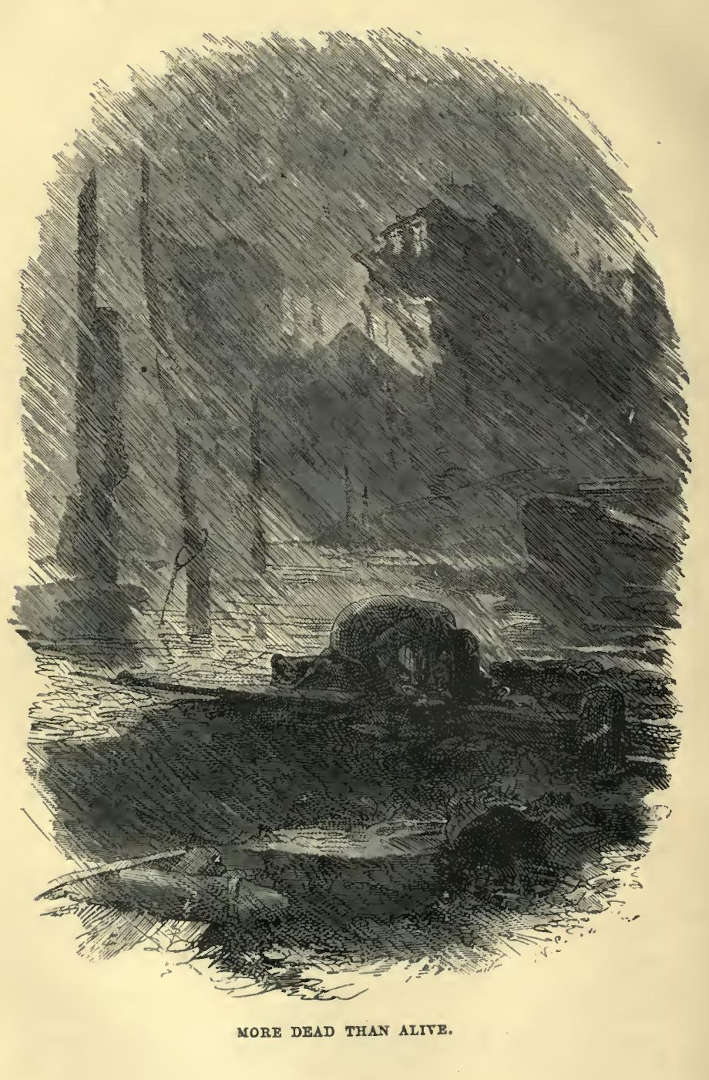
\includegraphics[scale=2.3]{02-13-01}

‘That night I almost gave up my mystery, though I suspected no one,
could offer no information, knew absolutely nothing save that the
murdered man was not I, but Radfoot. Next day while I hesitated, and
next day while I hesitated, it seemed as if the whole country were
determined to have me dead. The Inquest declared me dead, the Government
proclaimed me dead; I could not listen at my fireside for five minutes
to the outer noises, but it was borne into my ears that I was dead.

‘So John Harmon died, and Julius Handford disappeared, and John
Rokesmith was born. John Rokesmith’s intent to-night has been to repair
a wrong that he could never have imagined possible, coming to his ears
through the Lightwood talk related to him, and which he is bound by
every consideration to remedy. In that intent John Rokesmith will
persevere, as his duty is.

‘Now, is it all thought out? All to this time? Nothing omitted? No,
nothing. But beyond this time? To think it out through the future, is a
harder though a much shorter task than to think it out through the past.
John Harmon is dead. Should John Harmon come to life?

‘If yes, why? If no, why?’

‘Take yes, first. To enlighten human Justice concerning the offence of
one far beyond it who may have a living mother. To enlighten it with the
lights of a stone passage, a flight of stairs, a brown window-curtain,
and a black man. To come into possession of my father’s money, and with
it sordidly to buy a beautiful creature whom I love--I cannot help it;
reason has nothing to do with it; I love her against reason--but who
would as soon love me for my own sake, as she would love the beggar at
the corner. What a use for the money, and how worthy of its old misuses!

‘Now, take no. The reasons why John Harmon should not come to life.
Because he has passively allowed these dear old faithful friends to pass
into possession of the property. Because he sees them happy with it,
making a good use of it, effacing the old rust and tarnish on the money.
Because they have virtually adopted Bella, and will provide for her.
Because there is affection enough in her nature, and warmth enough in
her heart, to develop into something enduringly good, under favourable
conditions. Because her faults have been intensified by her place in my
father’s will, and she is already growing better. Because her marriage
with John Harmon, after what I have heard from her own lips, would be a
shocking mockery, of which both she and I must always be conscious, and
which would degrade her in her mind, and me in mine, and each of us in
the other’s. Because if John Harmon comes to life and does not marry
her, the property falls into the very hands that hold it now.

‘What would I have? Dead, I have found the true friends of my lifetime
still as true as tender and as faithful as when I was alive, and making
my memory an incentive to good actions done in my name. Dead, I have
found them when they might have slighted my name, and passed
greedily over my grave to ease and wealth, lingering by the way, like
single-hearted children, to recall their love for me when I was a poor
frightened child. Dead, I have heard from the woman who would have been
my wife if I had lived, the revolting truth that I should have purchased
her, caring nothing for me, as a Sultan buys a slave.

‘What would I have? If the dead could know, or do know, how the living
use them, who among the hosts of dead has found a more disinterested
fidelity on earth than I? Is not that enough for me? If I had come back,
these noble creatures would have welcomed me, wept over me, given up
everything to me with joy. I did not come back, and they have passed
unspoiled into my place. Let them rest in it, and let Bella rest in
hers.

‘What course for me then? This. To live the same quiet Secretary life,
carefully avoiding chances of recognition, until they shall have become
more accustomed to their altered state, and until the great swarm of
swindlers under many names shall have found newer prey. By that time,
the method I am establishing through all the affairs, and with which I
will every day take new pains to make them both familiar, will be, I may
hope, a machine in such working order as that they can keep it going.
I know I need but ask of their generosity, to have. When the right time
comes, I will ask no more than will replace me in my former path of
life, and John Rokesmith shall tread it as contentedly as he may. But
John Harmon shall come back no more.

‘That I may never, in the days to come afar off, have any weak misgiving
that Bella might, in any contingency, have taken me for my own sake if
I had plainly asked her, I WILL plainly ask her: proving beyond all
question what I already know too well. And now it is all thought out,
from the beginning to the end, and my mind is easier.’


So deeply engaged had the living-dead man been, in thus communing with
himself, that he had regarded neither the wind nor the way, and had
resisted the former instinctively as he had pursued the latter. But
being now come into the City, where there was a coach-stand, he stood
irresolute whether to go to his lodgings, or to go first to Mr Boffin’s
house. He decided to go round by the house, arguing, as he carried his
overcoat upon his arm, that it was less likely to attract notice if left
there, than if taken to Holloway: both Mrs Wilfer and Miss Lavinia being
ravenously curious touching every article of which the lodger stood
possessed.

Arriving at the house, he found that Mr and Mrs Boffin were out, but
that Miss Wilfer was in the drawing-room. Miss Wilfer had remained at
home, in consequence of not feeling very well, and had inquired in the
evening if Mr Rokesmith were in his room.

‘Make my compliments to Miss Wilfer, and say I am here now.’

Miss Wilfer’s compliments came down in return, and, if it were not too
much trouble, would Mr Rokesmith be so kind as to come up before he
went?

It was not too much trouble, and Mr Rokesmith came up.

Oh she looked very pretty, she looked very, very pretty! If the father
of the late John Harmon had but left his money unconditionally to his
son, and if his son had but lighted on this loveable girl for himself,
and had the happiness to make her loving as well as loveable!

‘Dear me! Are you not well, Mr Rokesmith?’

‘Yes, quite well. I was sorry to hear, when I came in, that YOU were
not.’

‘A mere nothing. I had a headache--gone now--and was not quite fit for
a hot theatre, so I stayed at home. I asked you if you were not well,
because you look so white.’

‘Do I? I have had a busy evening.’

She was on a low ottoman before the fire, with a little shining jewel
of a table, and her book and her work, beside her. Ah! what a different
life the late John Harmon’s, if it had been his happy privilege to take
his place upon that ottoman, and draw his arm about that waist, and say,
‘I hope the time has been long without me? What a Home Goddess you look,
my darling!’

But, the present John Rokesmith, far removed from the late John Harmon,
remained standing at a distance. A little distance in respect of space,
but a great distance in respect of separation.

‘Mr Rokesmith,’ said Bella, taking up her work, and inspecting it all
round the corners, ‘I wanted to say something to you when I could have
the opportunity, as an explanation why I was rude to you the other day.
You have no right to think ill of me, sir.’

The sharp little way in which she darted a look at him, half sensitively
injured, and half pettishly, would have been very much admired by the
late John Harmon.

‘You don’t know how well I think of you, Miss Wilfer.’

‘Truly, you must have a very high opinion of me, Mr Rokesmith, when you
believe that in prosperity I neglect and forget my old home.’

‘Do I believe so?’

‘You DID, sir, at any rate,’ returned Bella.

‘I took the liberty of reminding you of a little omission into which you
had fallen--insensibly and naturally fallen. It was no more than that.’

‘And I beg leave to ask you, Mr Rokesmith,’ said Bella, ‘why you took
that liberty?--I hope there is no offence in the phrase; it is your own,
remember.’

‘Because I am truly, deeply, profoundly interested in you, Miss Wilfer.
Because I wish to see you always at your best. Because I--shall I go
on?’

‘No, sir,’ returned Bella, with a burning face, ‘you have said more than
enough. I beg that you will NOT go on. If you have any generosity, any
honour, you will say no more.’

The late John Harmon, looking at the proud face with the down-cast eyes,
and at the quick breathing as it stirred the fall of bright brown hair
over the beautiful neck, would probably have remained silent.

‘I wish to speak to you, sir,’ said Bella, ‘once for all, and I don’t
know how to do it. I have sat here all this evening, wishing to speak to
you, and determining to speak to you, and feeling that I must. I beg for
a moment’s time.’

He remained silent, and she remained with her face averted, sometimes
making a slight movement as if she would turn and speak. At length she
did so.

‘You know how I am situated here, sir, and you know how I am situated
at home. I must speak to you for myself, since there is no one about
me whom I could ask to do so. It is not generous in you, it is not
honourable in you, to conduct yourself towards me as you do.’

‘Is it ungenerous or dishonourable to be devoted to you; fascinated by
you?’

‘Preposterous!’ said Bella.

The late John Harmon might have thought it rather a contemptuous and
lofty word of repudiation.

‘I now feel obliged to go on,’ pursued the Secretary, ‘though it were
only in self-explanation and self-defence. I hope, Miss Wilfer, that
it is not unpardonable--even in me--to make an honest declaration of an
honest devotion to you.’

‘An honest declaration!’ repeated Bella, with emphasis.

‘Is it otherwise?’

‘I must request, sir,’ said Bella, taking refuge in a touch of timely
resentment, ‘that I may not be questioned. You must excuse me if I
decline to be cross-examined.’

‘Oh, Miss Wilfer, this is hardly charitable. I ask you nothing but what
your own emphasis suggests. However, I waive even that question. But
what I have declared, I take my stand by. I cannot recall the avowal of
my earnest and deep attachment to you, and I do not recall it.’

‘I reject it, sir,’ said Bella.

‘I should be blind and deaf if I were not prepared for the reply.
Forgive my offence, for it carries its punishment with it.’

‘What punishment?’ asked Bella.

‘Is my present endurance none? But excuse me; I did not mean to
cross-examine you again.’

‘You take advantage of a hasty word of mine,’ said Bella with a little
sting of self-reproach, ‘to make me seem--I don’t know what. I spoke
without consideration when I used it. If that was bad, I am sorry; but
you repeat it after consideration, and that seems to me to be at least
no better. For the rest, I beg it may be understood, Mr Rokesmith, that
there is an end of this between us, now and for ever.’

‘Now and for ever,’ he repeated.

‘Yes. I appeal to you, sir,’ proceeded Bella with increasing spirit,
‘not to pursue me. I appeal to you not to take advantage of your
position in this house to make my position in it distressing and
disagreeable. I appeal to you to discontinue your habit of making your
misplaced attentions as plain to Mrs Boffin as to me.’

‘Have I done so?’

‘I should think you have,’ replied Bella. ‘In any case it is not your
fault if you have not, Mr Rokesmith.’

‘I hope you are wrong in that impression. I should be very sorry to
have justified it. I think I have not. For the future there is no
apprehension. It is all over.’

‘I am much relieved to hear it,’ said Bella. ‘I have far other views in
life, and why should you waste your own?’

‘Mine!’ said the Secretary. ‘My life!’

His curious tone caused Bella to glance at the curious smile with which
he said it. It was gone as he glanced back. ‘Pardon me, Miss Wilfer,’
he proceeded, when their eyes met; ‘you have used some hard words, for
which I do not doubt you have a justification in your mind, that I do
not understand. Ungenerous and dishonourable. In what?’

‘I would rather not be asked,’ said Bella, haughtily looking down.

‘I would rather not ask, but the question is imposed upon me. Kindly
explain; or if not kindly, justly.’

‘Oh, sir!’ said Bella, raising her eyes to his, after a little struggle
to forbear, ‘is it generous and honourable to use the power here which
your favour with Mr and Mrs Boffin and your ability in your place give
you, against me?’

‘Against you?’

‘Is it generous and honourable to form a plan for gradually bringing
their influence to bear upon a suit which I have shown you that I do not
like, and which I tell you that I utterly reject?’

The late John Harmon could have borne a good deal, but he would have
been cut to the heart by such a suspicion as this.

‘Would it be generous and honourable to step into your place--if you did
so, for I don’t know that you did, and I hope you did not--anticipating,
or knowing beforehand, that I should come here, and designing to take me
at this disadvantage?’

‘This mean and cruel disadvantage,’ said the Secretary.

‘Yes,’ assented Bella.

The Secretary kept silence for a little while; then merely said, ‘You
are wholly mistaken, Miss Wilfer; wonderfully mistaken. I cannot say,
however, that it is your fault. If I deserve better things of you, you
do not know it.’

‘At least, sir,’ retorted Bella, with her old indignation rising, ‘you
know the history of my being here at all. I have heard Mr Boffin say
that you are master of every line and word of that will, as you are
master of all his affairs. And was it not enough that I should have been
willed away, like a horse, or a dog, or a bird; but must you too begin
to dispose of me in your mind, and speculate in me, as soon as I had
ceased to be the talk and the laugh of the town? Am I for ever to be
made the property of strangers?’

‘Believe me,’ returned the Secretary, ‘you are wonderfully mistaken.’

‘I should be glad to know it,’ answered Bella.

‘I doubt if you ever will. Good-night. Of course I shall be careful to
conceal any traces of this interview from Mr and Mrs Boffin, as long as
I remain here. Trust me, what you have complained of is at an end for
ever.’

‘I am glad I have spoken, then, Mr Rokesmith. It has been painful and
difficult, but it is done. If I have hurt you, I hope you will forgive
me. I am inexperienced and impetuous, and I have been a little spoilt;
but I really am not so bad as I dare say I appear, or as you think me.’

He quitted the room when Bella had said this, relenting in her wilful
inconsistent way. Left alone, she threw herself back on her ottoman, and
said, ‘I didn’t know the lovely woman was such a Dragon!’ Then, she
got up and looked in the glass, and said to her image, ‘You have been
positively swelling your features, you little fool!’ Then, she took an
impatient walk to the other end of the room and back, and said, ‘I
wish Pa was here to have a talk about an avaricious marriage; but he
is better away, poor dear, for I know I should pull his hair if he WAS
here.’ And then she threw her work away, and threw her book after
it, and sat down and hummed a tune, and hummed it out of tune, and
quarrelled with it.

And John Rokesmith, what did he?

He went down to his room, and buried John Harmon many additional fathoms
deep. He took his hat, and walked out, and, as he went to Holloway or
anywhere else--not at all minding where--heaped mounds upon mounds of
earth over John Harmon’s grave. His walking did not bring him home until
the dawn of day. And so busy had he been all night, piling and piling
weights upon weights of earth above John Harmon’s grave, that by that
time John Harmon lay buried under a whole Alpine range; and still the
Sexton Rokesmith accumulated mountains over him, lightening his labour
with the dirge, ‘Cover him, crush him, keep him down!’



